\chapter{Background}
%%%%%%%%%%%%%%%%%%%%%%%%%%%%%%%%%%%%%%%%%%%%%%%%%%%%%%%%%%%%%%%%%%%%%%%%%%%%%%%%%%%%
%###################################################################################
Distributed software development (\ac{dsd}) is today practiced commonly in the software industry in both large and small companies and organizations \citep{shrivastava2010distributed}. This means that software development teams are not physically sitting in the same place and hence don’t have the opportunity to meet or speak to other team members in person regularly \citep{layman2006essential}. This distribution might mean sitting in two different buildings or sitting on two different continents. \ac{gsd} is a particular form of \ac{dsd} in which the distribution of teams are across national borderlines \citep{sahay2003global}. 

Communication has an important role in the success of \ac{gsd} \citep{carmel2001tactical,french1998study}, especially informal communication \citep{herbsleb2003empirical}. The processes of communication, coordination, and collaboration are of the utmost importance and key aspects of the software development process \citep{colomo2014agile}. 

Research shows that distance has a significant impact on the performance of projects \citep{damian2003global,Herbsleb2001a}. Communication is also an essential part of all software development practices \citep{layman2006essential}. Empirical research also shows that developers are in need of ad hoc and informal communication \citep{grinter1998recomposition,kraut1995coordination}. Therefore any shortcomings in communication between the teams and team members will profoundly impact the success of \ac{gsd} projects \citep{layman2006essential}.

Face-to-face meetings are the most efficient and ideal type of communication \citep{Kirkman2004}, but in \ac{gsd} which teams are spread in different places, often with time zone differences, this is not possible and therefore might be challenging to achieve effective communication between teams and team members. In the presence of temporal distance between the teams and team members real-time and synchronous communication using a phone, and text or video chat is challenging to achieve \citep{holmstrom2006agile,kommeren2007philips}.

\citet{casey2008impact} have worked on a case in which two distributed teams located in Ireland and Malaysia used just an asynchronous type of communication, e-mail. In that case, using asynchronous communication tools, like e-mail increased the chances of misunderstanding and ambiguity of information. Also, the communication is not adequate if the parties communicating with each other don’t understand each other \citep{kommeren2007philips,cataldo2007coordination}.

Receiving delayed feedback is also another challenge faced by remotely located teams, which itself is again a side effect of asynchronous communication \citep{conchuir2006exploring,holmstrom2006agile}. Research shows that using asynchronous communication tools in remote teams increases dramatically the time it takes to receive a response \citep{holmstrom2006global}. 

It is also true that a software engineer usually spends most of her time in searching and exchanging information, rather than doing anything else, and as a result, this can lead to delays in completing the project and increases the cost of the project. One of the ways to mitigate this problem is through proper project coordination \citep{dumitriu2006issues}. \hl{why synchronous is essential (last 2 paragraphs are about it)}

%%%%%%%%%%%%%%%%%%%%%%%%%%%%%%%%%%%%%%%%%%%%%%%%%%%%%%%%%%%%%%%%%%%%%%%%%%%%%%%%%%%%%%%%%%%%%%%%%%
\section{Coordination} \label{coordinering}
%%%%%%%%%%%%%%%%%%%%%%%%%%%%%%%%%%%%%%%%%%%%%%%%%%%%%%%%%%%%%%%%%%%%%%%%%%%%%%%%%%%%%%%%%%%%%%%%%%
Scholars have defined coordination in different ways. \citet{Malone1988} defines coordination as for when several actors seek goals together and must do things to organize themselves in order to reach that goal while a single actor seeking the same goals does not have to do the same things. He calls these extra activities needed for organizing, coordination. Later, \citet{Malone1994} adjusted the definition of coordination to managing of dependencies. The definition is justified in that there are interdependent associations between activities, and contrive with these relations effectively, coordination mechanisms are needed \citep{Deng2007}.

Coordination from Osifo's (2012) point of view can be classified as part of an organization. At the same time, \citep{Beuselinck2007} and \citep{Osifo2012} confirm Malone and Crowston’s (\citeyear{Malone1988}) definition which states that there would be no need for coordination if there is no dependency and relation.

There are two aspects of the coordination which are important for organizations, internal and external coordination. Internal coordination is important to achieve cooperation by having support and clarity. Without internal coordination, it would be difficult to achieve satisfactory progress in the projects. It also provides help in setting rules and criteria. External coordination also plays an important role in setting limits so that the project always stays in focus and continues on the right path \citep{Osifo2012}.

Coordination is part of nearly every single part of a project and is rarely employed alone by only one coordination mechanism \citep{Osifo2012}. Almost always coordination of a particular project or organization is accomplished by using several coordination mechanisms \citep{Dietrich2013}.

%%%%%%%%%%%%%%%%%%%%%%%%%%%%%%%%%%%%%%%%%%%%%%%%%%%%%%%%%%%%%%%%%%%%%%%%%%%%%%%%%%%%%%%%%%%%%%%%%%
\subsection{Van de Ven model of coordination}
Researchers have suggested several coordination mechanisms. \citet{Strode2012} states that synchronization, structure, and boundary spanning are mechanisms which are worthy for efficient coordination. \citet{Mintzberg1980} believes that mechanisms such as mutual adjustment, direct supervision, and standardization are of importance in coordination.

\citet{VanDeVen1976} suggest another coordination model which is somehow similar to other scholars but adds the notion of team to the coordination strategy. For example, they believe that mutual adjustment in co-located teams is reached by mutual interactions.

\citet{VanDeVen1976} suggest another coordination model which is somehow similar to the models suggested by other scholars but adds the notion of team to the coordination strategy. For example, they believe that mutual adjustment in co-located teams is reached by mutual interactions.
Still, in the case of the ways in which coordination can be achieved it is somewhat similar to the theory suggested by  \citet{Thompson2014}. According to \citet{VanDeVen1976}, there are three modes for coordination of work activities; impersonal, personal, and group mode of coordination.

In Van de Van's model, the focus is on the team and how based on the change of some factors the coordination modes changes. \citet{VanDeVen1976} suggest that coordination mechanisms in every one of those three modes are utilized in different combinations to reach a certain collective goal.

%%%%%%%%%%%%%%%%%%%%%%%%%%%%%%%%%%%%%%%%%%%%%%%%%%%%%%%%%%%%%%%%%%%%%%%%%%%%%%%%%%%%%%%%%%%%%%%%%%
\subsection{Impersonal mode of coordination}
Anything that needs the minimum amount of verbal communication between actors once implemented and in nature is relevant to programming, technical means, and administrative coordination can be correlated with impersonal mode of coordination \citep{Boos2011,VanDeVen1976}.

\citet{Kraut1995a} suggest some coordination techniques that can reduce some of the coordination challenges when a mixture of large size, intricacy, and interdependence occurs simultaneously;  using technical tools, modularization, and formal procedures are some of the suggested techniques.

Keeping large-scale projects coordinated by using tools and having a shared system to keep the record of documents is of utmost importance. Some of the examples of impersonal coordination mechanisms found in large-scale agile are standardization of work process (such as following the scrum methodology), having rules for QA, and use of tools such as Jira \citep{Nyrud2017b}.
%%%%%%%%%%%%%%%%%%%%%%%%%%%%%%%%%%%%%%%%%%%%%%%%%%%%%%%%%%%%%%%%%%%%%%%%%%%%%%%%%%%%%%%%%%%%%%%%%%
\subsection{Personal mode of coordination}
In the personal mode, according to \citet{VanDeVen1976}, coordination happens through feedback or mutual adjustments on the input information that an actor receives from the other actors. Mutual task adjustments happen either through vertical or horizontal communication channels.
Line managers and unit supervisors are often the mechanisms of vertical communication which is hierarchical in nature \citep{Thompson2014}. But horizontal communication is more about individual people in teams that communicate on a one-to-one basis with other team members, and it is usually non-hierarchical \citep{VanDeVen1976}.

\citet{Mintzberg1980} divides coordination mechanisms to mutual adjustment and direct supervision. These two mechanisms are similar to vertical and horizontal channels of communication in the personal mode of coordination. Mutual adjustment happens when people in the team informally communicate with other teammates to coordinate their tasks. In the direct supervision, a person from a higher level than the others, like the head of a team, gives some instructions that must be followed by other team members who work under her supervision.
\hl{Hva er egentlig IM? A tool? Impersonal. Mutual adjustment -> vertical/horizontal personal mode? 1to1 group mode unscheduled? channels.}

Personal mode of coordination consists of both informal and formal communication \citep{Kraut1995a}. Also, it is more valuable in unscheduled and unexpected encounters \citep{Boos2011,Dickenson1997}. \citet{Kraut1995a} suggest that informal communication between team members while discussing work-related matters in front of water or coffee machine forms a large amount of coordination and that coordination does not only happen in formal meetings.

The success of coordination is dependent on some factors. Trust is one of those factors because organizational performance is realized by the network created by coordination \citep{DeJong2016}. Reduced coordination is in direct association with trust \citep{RoohullahJan2016}. And its importance is because it is the central part of decent coordination \citep{Osifo2012}. 

%%%%%%%%%%%%%%%%%%%%%%%%%%%%%%%%%%%%%%%%%%%%%%%%%%%%%%%%%%%%%%%%%%%%%%%%%%%%%%%%%%%%%%%%%%%%%%%%%%
\subsection{Group mode of coordination}
Group mode of coordination, like the personal mode, happens by feedback and mutual adjustments but with the difference that all these happen in the group in unscheduled or scheduled meetings and consists of more planned communication \citep{VanDeVen1976}.

\citet{Dietrich2013} suggest three other coordination mechanisms that are important in large-scale projects. Those three mechanisms are called centralized, decentralized, and balanced patterns, which respectively are about coordination at the group level that is either scheduled or unscheduled, coordination between teammates which are not scheduled, and at last the combination of the first two ones.

The coordination strategy that \citet{Strode2012} have suggested involves three principal concepts of synchronization, structure, and boundary spanning that assist in managing dependencies. Regarding the group mode of coordination, synchronization has more relevance and importance and is gained within synchronization activities. These activities are done usually once at the beginning of the project, but also can happen several times during the project so that the team members are aware of the project requirements and maintain this understanding during the whole project \citep{Strode2012}.

%%%%%%%%%%%%%%%%%%%%%%%%%%%%%%%%%%%%%%%%%%%%%%%%%%%%%%%%%%%%%%%%%%%%%%%%%%%%%%%%%%%%%%%%%%%%%%%%%%
\section{Communication} \label{communication}
%%%%%%%%%%%%%%%%%%%%%%%%%%%%%%%%%%%%%%%%%%%%%%%%%%%%%%%%%%%%%%%%%%%%%%%%%%%%%%%%%%%%%%%%%%%%%%%%%%
All team members in both collocated and distributed software teams communicate with each other using some form of Internet-based communication tool \citep{Kirkman2005}. Using internet-based communication in teams have several benefits for companies, such as easier access to the global market, preserving the environment, and having team members in different locations around the globe that will enable the companies to work non-stop \citep{Cascio2000}. Research also shows that distributed teams, that are inevitably using internet-based communication, performing better than traditional teams in tasks like brainstorming because of the elimination of production blocking effects \citep{Espinosa2015}.

However, there are some challenges that threats distributed teams. High pressure in mastering advanced communication technology and lack of nonverbal communication, as well as problems in forming trust are some of them \citep{Jarvenpaa1998,Kayworth2002}. Misunderstanding might also happen easily in the absence of sentiment and meta-level information, such as body language \citep{Cramton2001}. Although the type of communication technology and tools will affect the communication in teams and might lead to limited information sharing between distributed team members \citep{Gilson2015}.

%%%%%%%%%%%%%%%%%%%%%%%%%%%%%%%%%%%%%%%%%%%%%%%%%%%%%%%%%%%%%%%%%%%%%%%%%%%%%%%%%%%%%%%%%%%%%%%%%%
\subsection{Media Richness and Media Synchronicity Theories}
Seminal media theory tries to categorize the communication media based on their effectiveness and "richness" to express the link between communication and technology, and in this regard sees the richest medium in face-to-face encounters that is able of carrying all the verbal and non-verbal messages and minimizes the ambiguity while sees the written mediums, such as email, as the least rich medium of communication \citep{Daft1986,Hassell2016}.

Later, \citet{Dennis2008} proposed the Media synchronicity theory to address the limitations and shortcomings of the other media theory proposed before. Media synchronicity theory discusses the different attributes of several types of media and attempts to look at them more precisely.

\citet{Dennis2008} suggest five attributes:

1- Regardless of the medium to be synchronous or asynchronous, immediate feedback is present.\\
2- Availability and diversity of symbols.\\
3- Availability of the ability to have several parallel conversations at the same time.\\
4- The messages can be rehearsed before transmission.\\
5- The conversations and messages sent and received can be retrieved.\\

\hl{Figure 1. Breakdown of communication media according to the criteria proposed by the media synchronicity theory. (Maruping and Agarwal, 2004) }

%%%%%%%%%%%%%%%%%%%%%%%%%%%%%%%%%%%%%%%%%%%%%%%%%%%%%%%%%%%%%%%%%%%%%%%%%%%%%%%%%%%%%%%%%%%%%%%%%%
\subsection{Enterprise Social Networks}
Because of the value that organizations see in using social media at the workplace and high demand for such platforms, during the recent years, several companies have started to develop tools such as Slack, HipChat, Yammer, and Workplace by Facebook \citep{Leroy2013}. These applications are known as Social Networking Platforms (SNP) or Team Communication Platforms (TCP), and can be categorized under communication methods that are called enterprise Social Networking (ESN) or Enterprise Social Media (ESM).

One thing that differentiates usual social media such as Facebook and Twitter from ESN is that social media is open to public and everyone can use them but access to ESN is limited to employees and those whom the company needs to get in touch with them regularly \citep{Turban2011}.

\citet{Leonardi2013} describe four attributes which a platform should provide for its users to be considered as an ESN:\\
1- The users must be able to send and receive messages to individual members as well as the whole or a group of members. \\
2- Either explicitly or implicitly should be able to choose and show special coworkers as their communication partners.\\
3- It must be possible to share files with other users.\\
4- At any time it must be possible for any user to view all the conversations that are done publicly, consisting of text messages and file shared.

ESN acts as a forum for its members where they are able to communicate with other co-workers in the same organization \citep{Leonardi2014} in which business goals, such as enhanced knowledge sharing, easier access to expertise, and innovation can be reached better in a more secure and private environment \citep{Leonardi2013}.

If the ESN is correctly managed it can boost the productivity and motivation of employees, enhance collaboration between the different actors in the organization, and lead to more learning for team members \citep{Leon2017}. It also enables people in different locations to be able to communicate and become involve in innovation, revenue creation, and socio-economic growth \citep{Qi2016}.

One of the problems that can be associated with the long-term use of ESNs is that employees might feel isolated because of limited face-to-face encounters with other people \citep{Kane2014}, but at the same time ESN is not designed and meant to completely replace personal and physical encounters \citep{Zhang2013a}.

Also because of the learning curve associated with any new tool, organizations might have not completely reached their goals in increasing collaboration between their employees \citep{Anderson2016}. However, developing an open culture among the employees and using an ESN which have similarities to social media that employees use in their private life may help to improve the usage of ESN by employees \citep{Korzynski2014}. 

%%%%%%%%%%%%%%%%%%%%%%%%%%%%%%%%%%%%%%%%%%%%%%%%%%%%%%%%%%%%%%%%%%%%%%%%%%%%%%%%%%%%%%%%%%%%%%%%%%
\section{Distributed teams} \label{dt}
%%%%%%%%%%%%%%%%%%%%%%%%%%%%%%%%%%%%%%%%%%%%%%%%%%%%%%%%%%%%%%%%%%%%%%%%%%%%%%%%%%%%%%%%%%%%%%%%%%
Distributed teams are called by several names, but it is generally agreed that a team is considered as distributed when its members are spread at least in two locations \citep{Hinds2005}. This physical separation can range between two different offices in the same city or country or people sitting in different countries and continents \citep{Mortensen2001}. Here I will now discuss some of the advantages and disadvantages of using distributed software teams.
%%%%%%%%%%%%%%%%%%%%%%%%%%%%%%%%%%%%%%%%%%%%%%%%%%%%%%%%%%%%%%%%%%%%%%%%%%%%%%%%%%%%%%%%%%%%%%%%%%
\subsection{Advantages of using distributed teams}
When evaluating distributed teams and discussing the dynamic situation of global business it is essential to know the advantages that this type of team structure offers a company that uses it. 

1- Companies can benefit from a much more bigger pool of global experts in different subjects and recruit some of the best talents that might not be available locally or might be expensive to recruit \citep{Snyder2003}. Relocation is costly and stressful and today most of the workers try to avoid it \citep{Lipnack1997,Joinson2002}. Human resources of companies can be increased in this case, because especially skilled members of the company can serve on several teams simultaneously \citep{Hertel2004}. 

2- Costs associated with traveling and accommodation will be reduced drastically or completely eliminated. \citet{Baskerville2007} report that IBM by using distributed teams saved \$50 million in travel and downtime costs.

3- Distributed teams encourages multiculturalism and discourages discrimination by age and race because the members are evaluated by the performance and productivity. This type of team fosters equality and fairness among the employees \citep{Bergiel2007}.

4- Because of the diversity and heterogeneity of distributed teams, these teams are more effective and promote creativity among its members compared to more rigid structure of traditional teams which are limited by time and space \citep{Bergiel2008}.
%%%%%%%%%%%%%%%%%%%%%%%%%%%%%%%%%%%%%%%%%%%%%%%%%%%%%%%%%%%%%%%%%%%%%%%%%%%%%%%%%%%%%%%%%%%%%%%%%%
\subsection{Disadvantages of using distributed teams}
1- Managing conflicts between team members in distributed teams is a big challenge \citep{Hinds2003}. Lack of good communication tools and a shared identity in distributed teams lead to conflict \citep{Hinds2005a}. 

2- Coordination and cohesion may be reduced in distributed teams which in turn affects work performance \citep{DeRosa2004}.

3- Feeling isolated and lack of face-to-face social interaction is also common in distributed teams that don't have the opportunity of meeting their colleagues as often as traditional teams \citep{Kiesler2002}.

%%%%%%%%%%%%%%%%%%%%%%%%%%%%%%%%%%%%%%%%%%%%%%%%%%%%%%%%%%%%%%%%%%%%%%%%%%%%%%%%%%%%%%%%%%%%%%%%%%
\section{Slack} \label{slack}
%%%%%%%%%%%%%%%%%%%%%%%%%%%%%%%%%%%%%%%%%%%%%%%%%%%%%%%%%%%%%%%%%%%%%%%%%%%%%%%%%%%%%%%%%%%%%%%%%%
Since analyzing Slack constitutes an important part of this thesis and Slack is more than yet another chat application I decided to give a description of this platform and some of its most important functions that makes Slack one of the most popular communication and collaboration systems used in software teams.

In order to describe Slack both secondary data obtained from its website, as well as my own experience as a lack user is used. The reader of this introduction will get a sense of what Slack, as a sophisticated enterprise social network is.

Slack was started in 2013 and has more than eight million active users every day, three million of which are paid users \citep{Lynley2018}. It has turned a contemporary form of communication, i.e texting, into a workplace app. Its valuation is \$ 5.1 billion. Although it has recently encountered by some big players in the market, like Microsoft, Google, and Facebook, still 43 percent of Fortune 100 companies are using Slack. Its popularity among startup companies is the same, if not more than the big enterprises \citep{Rodriguez2018}.

\citet{Williams2015a} who has created a document on how to use the Slack, says that Slack can be seen as a chat room where the whole company and its different teams can be broken into smaller channels for group discussion. Channels are often created to discuss a certain topic and are like the old chat rooms. Like any other communication platform, sending direct messages to individuals is also possible in Slack.

Slack is a multi-platform software, meaning that it can be used on all kinds of operating systems on all mobile phones, as well as desktops and laptops. The user can be notified of several things by several ways. Direct messages and mentions usually generate notifications that can both received by email, if the user is not online, or will be shown on the Slack app. These notifications are highly customizable and can be suppressed to avoid being overwhelmed by the number of notifications. 

Teams are another feature of Slack. Groups of people who are working together can use it to communicate with each other. It can be created simply by visiting Slack's website. A team must have an owner and can have several admins who will enforce the team rules. Often working in large organizations means being part of several Slack teams. There is also possible to work in several workspaces, as each one works as a separate team that is connected to the Slack's enterprise network.  All the teams and works places are available on the web, desktop, and mobile version of Slack.

Figure \ref{fig:slack} shows an screen shot of a Slack channel.
\begin{figure}[hbt!]
\centering
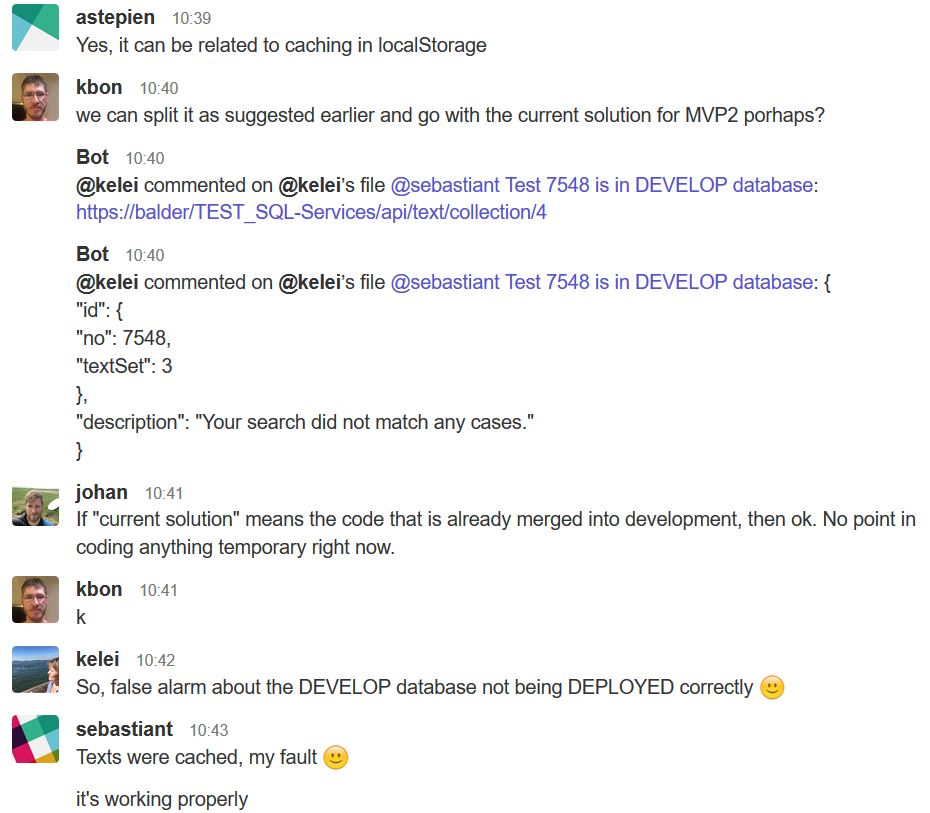
\includegraphics[width=\linewidth, frame]{slack.JPG}
\caption{A screenshot from Slack}\label{fig:slack}
\index{figures}
\end{figure}


Channels in Slack are used as chat rooms for group conversation. Different channels are usually created to discuss certain topics. These channels can either be public or private. Public channels are visible to the entire team and all the team members can join them. But private channels need an invitation to join and usually, admin of the channels adds the other users to the channel.
 
Everything shared on Slack, including text, image, file, and other types of posts can be searched by users. The information shared in private channels can just be searched and found by the members of the channel. Also paid customers of Slack have the ability to invite external users. In that case, only the information shared in the respective channels can be searched and found by the external member.

The other way that users can communicate in Slack is by direct messages (DM). It is possible to send a DM to up to eight other users simultaneously. Obviously, these messages can be just seen and searched by those who are involved in the messages. It is also possible to call up to fifteen users at the same time if the team is a using the paid service, but in the free version, just one-on-one calls are supported. 

Using emoji is another way of communicating in Slack, it can be both used by the user who is writing the message to communicate her emotions (Figure \ref{fig:slack}), as well as by the readers of the message who can "react" to the message and communicate their emotion with the sender of the message. it is also common to get the attention of someone or the whole members of a channel by putting @ before the username of the users. In this case, users will immediately get a notification if they are online, or will get an email in case they are offline.

Moreover, the notifications that the user receives can be heavily customized to meet the needs of the user. Users, for example, may define certain words and phrases that when appeared in chat messages visible by the user the system will generate a notification. Notification can be manipulated based on several properties, like time, date and location. For example, one can decide not to receive any notification during weekends. Another capability that Slack users have is the ability to organize messages by pinning them or starring them, in order to get access to important messages more easily late on. All the sent messages can also be edited after being sent. And the appearance of the Slack can be customized by changing themes and colors to match the taste of every individual user. 

One of the reasons that Slack is so popular in teams is because of its ability to integrate with lots of external services, like Google Calendar, GitHub, IFTTT, and many more \citep{Williams2015}. Users also have the possibility of sending and sharing files and folders. It is also possible for users to make voice and video calls. All the function mentioned in this section are provided free of charge but enterprise users can pay to enjoy some extra features like group video chats, more storage, and unlimited availability of past conversations. \hl{Good, but can it be related to theory in the pic1(maruping 2004)? Slack also has editability that can be added to the theory. Slack also has rehearsability.}
